% ++++++++++++ Domain Pi AKS klassen ++++++++++++++

\vfill
\subsubsection{Domain-klasse: Aks}\label{sec:aks_design}

\begin{figure}[h]
\centering
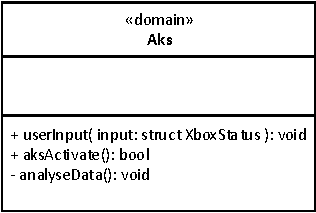
\includegraphics[scale=1]{../fig/diagrammer/bil/cd_aks.pdf}
\caption{Klassebeskrivelse for controller -klassen Aks}
\label{fig:cd_aks}
\end{figure}

Dette afsnit afspejler Aks, som den er implementeret i systemet ved aflevering af denne projektdokumentation og indeholder derved ikke nogle af de funktionaliteten, som er stillet i Kravspecifikationen.
Dette indebærer eksempelvis hvorvidt AKS er i stand til at dreje forbi en forhindring og ikke blot bremse. Det indebærer også funktionalitet til at bringe bilen helt til standsning ved en forhindring og ikke blot bremse momentant.

\clearpage

\textbf{Attributter}

\begin{table}[h]
\begin{tabularx}{\textwidth}{| Z | Z | L{9cm} |} \hline
Navn & Type & Beskrivelse \\\hline
\texttt{MySteering} & \texttt{Steering} & Styretøjsklassen, bruges når AKS skal påvirke bilens hastighed eller retning.\\\hline
\texttt{MyData} & \texttt{Data*} & Pointer til bilens datastruktur.\\\hline
\texttt{MySettings} & \texttt{Settings*} & Pointer til Settingsklassen. \\\hline
\texttt{MyLog} & \texttt{Log*} & Pointer til loggen. \\\hline
\texttt{state} & \texttt{aksStates} & Husker hvilket stadie bilen er i, kan skifte mellem at stå stille, køre fremad/bagud eller trille. \\\hline
\texttt{proxSensors} & \texttt{int*} & Et array med nuværende værdier fra afstandssensorer \\\hline
\texttt{old\_proxSensors} & \texttt{int*} & Et array der holder de foregående værdier fra afstandssensorer \\\hline
\texttt{latestUserInput} & \texttt{UserInput} & Gemmer de seneste input fra brugeren. \\ \hline
\end{tabularx}
\caption{Attributter for klassen Aks}
\label{table:attr_aks}
\end{table}

\textbf{Metoder}


%----------------- activate -------------------
\begin{table}[h]
\begin{tabularx}{\textwidth}{| L{2.5 cm} | Z |} \hline
Prototype & \texttt{void activate(void)} \\\hline
Parametre & \texttt{void}  \\\hline
Returværdi &  \texttt{void} \\\hline
Beskrivelse & Metoden indhenter data samt brugerinput og kalder analyseData kontinuert. Hvis der er behov for indgreb ifb. en eventuel kollision ignoreres input fra brugeren og activate genererer selv input til \texttt{Steering}, \\\hline
\end{tabularx}
\caption{Metodebeskrivelse for \texttt{activate}}
\label{table:met_aks_activate}
\end{table}

%----------------- analyseData -------------------
\begin{table}[h]
\begin{tabularx}{\textwidth}{| L{2.5 cm} | Z |} \hline
Prototype & \texttt{bool analyzeData(void)} \\\hline
Parametre & \texttt{void}  \\\hline
Returværdi &  \texttt{bool} \newline
Returnerer \texttt{true}, hvis der er behov for indgreb fra AKS, alternativt \texttt{false}, hvis der ikke er. \\\hline
Beskrivelse & Metoden analyserer indhentet data fra Data klassen og vurderer om der er en umiddelbar fare, som kræver et indgreb fra AKS. \\\hline
\end{tabularx}
\caption{Metodebeskrivelse for \texttt{analyzeData}}
\label{table:met_aks_analyzeData}
\end{table}